\documentclass{llncs}

\usepackage[utf8]{inputenc} %Aceita caracteres latinos

\usepackage{subfig}
\usepackage{graphicx,url}
\usepackage{amsmath, amssymb, exscale}          % Permite utilizar a parte AMS das formulas
\usepackage[normalem]{ulem}   % Permite sublinhar figuras
\usepackage{float}
\usepackage{algorithm2e}        % Para facilitar a escrita de Algoritmos
\usepackage{algorithmic}
\usepackage{booktabs}
\usepackage[disable]{todonotes}
\newcommand{\je}[2][]{\todo[color=pink, #1]{JE: {\small #2}} }
\usepackage{comment}
\usepackage{hyperref}
\usepackage{longtable}
\usepackage{enumerate}
\usepackage{microtype}
\usepackage{pgf}
\usepackage{tikz}
\usetikzlibrary{graphs}
\usetikzlibrary{arrows}
\usetikzlibrary{shapes}
\usetikzlibrary{fit}
\usetikzlibrary{trees}
\usetikzlibrary{plotmarks}
\usetikzlibrary{calc}
\usetikzlibrary{backgrounds}
\usetikzlibrary{intersections}
\usetikzlibrary{decorations.pathmorphing}
\usetikzlibrary{decorations.text}

\bibliographystyle{splncs04}

\hypersetup{
  colorlinks   = true, %Colours links instead of ugly boxes
  urlcolor     = blue, %Colour for external hyperlinks
  linkcolor    = black, %Colour of internal links
  citecolor    = black %Colour of citations
}

\newcommand{\clause}[1]{{\small\sffamily\color{black} #1}}

\usepackage{listings}
% This is to hace line numbers inside the text area
% https://tex.stackexchange.com/questions/68505/listings-line-numbers-and-figure
% Does not seem to work...
\lstset{numbers=left}
\makeatletter%
\def\lst@PlaceNumber{\makebox[\dimexpr 1em+\lst@numbersep][l]{\normalfont
  \lst@numberstyle{\thelstnumber}}}%
\makeatother%
\renewcommand\lstlistingname{Listing} % Change language of section name
\lstdefinestyle{prolog}{
aboveskip=2pt,belowskip=2pt,
	language=Prolog,
        basicstyle = \scriptsize\sffamily\color{black},
        %numbers=left,
        firstnumber=last,
        numberbychapter=false,
        captionpos=b,
        escapechar=|,
        escapeinside={(*}{*)},
        stepnumber=1,
        numberstyle=\tiny,
        showstringspaces=false,
        tabsize=1,
        breaklines=true,
        breakatwhitespace=false
        moredelim = [s][\color{black}]{(}{)},
        commentstyle=\color{green},
        keywordstyle=\color{blue},
        literate =
          {:-}{{\ttfamily\textcolor{blue}{:-}}}2
          {,}{{\ttfamily\textcolor{blue}{,}}}1
          {!}{{\ttfamily\textcolor{blue}{!}}}1
          {.}{{\ttfamily\textcolor{blue}{.}}}1
}
\lstdefinestyle{examples}{
	    style=prolog,
%        listingname=Examples, % not available
        numbers=none
}
\lstset{style=prolog}

\usepackage{pgfplots}
\usepackage{pgfplotstable}

% Add page numbers (fancyhdr may be used as well)
\pagestyle{headings} 
\begin{document}

\title{A Proposal for Optimizing Internetwork Matching of Ontologies}


\author{Fabio Santos, Kate Revoredo\thanks{Partially funded by Unirio (PQ-UNIRIO N01/2018)} and Fernanda Baião\thanks{Partially funded by CNPq (401505/2014-6)}}
\institute{
Department of Applied Informatics \\
Federal University of the State of Rio de Janeiro (Unirio), Rio de Janeiro, Brazil  \\
\email{\{fabio.santos, katerevoredo, fernanda.baiao\}@uniriotec.br} \\
}

\maketitle
\hyphenation{re-cog-ni-zed know-ledge me-cha-nisms exam-ples eva-lu-a-tion consi-dered exis-ting}
\begin{abstract}

A System-of-Systems (SoS) is a set of independent information systems that must communicate with each other towards providing a specific service. Therefore, effectively integrating these systems is demanding. Considering that each system is conceptually described by a unique ontology, the conceptual support for the whole SoS demands the alignment of all ontologies, deriving a network of ontologies. Existing ontology matching techniques may be used for the task; however, due to the recently increasing size of the ontologies and the potential number of ontologies being aligned, current approaches may suffer from scalability and performance issues. In this paper, we introduce an approach to reduce the number of potential correspondences, therefore optimizing the process of creating a network of ontologies. A preliminary experiment was conducted, showing the potential of the proposed approach. 
\end{abstract}

\keywords{network of ontologies \and network matching \and data integration}
\section{Introduction} \label{sec:introduction}

A System-of-Systems (SoS) is defined as a set of independent information systems (IS), providing functionalities derived from the interoperability among them \cite{boehm2006view}.
%\todo{aqui esta faltando referencia. de onde veio esta definicao? Coloquei.}.
The development and research on SoS have been gaining increasing attention due to the relevance of several domains such as smart cities, health, emergency response systems, and crisis management systems \cite{fitzgerald2013model}. \begin{comment}Conceptually, an SoS is defined by five characteristics \cite{maier1998architecting}: (i) \emph{managerial independence}, which states that each composing IS is under the responsibility of different organizations and managers; (ii) \emph{operational independence}, which states that each IS is able to proceed independently from the overall structure; (iii) \emph{distribution}, stating that ISs are connected to each other and collaborate towards a common goal; (iv) \emph{evolutionary development}, which states that the union of all ISs defines the SoS evolution; and (v) \emph{emergent behavior}, which states that new, intricate and huge features emerge from the SoS existence.  

In the nineties, an SoS has evolved to a System of Information Systems (SoIS) when a set of inter-operable IS exhibits all SoS characteristics with additional strong business nature", and more recently the term Smart System of Information Systems (Smart SoIS) appeared demanding full interoperability and dynamic architecture \cite{fitzgerald2013model}, which means self-* characteristics (self-adaptation, self-healing, and self-management) are presented, keeping the managements tasks easier than in previous SoS \cite{giese2015towards} 
\footnote{For the sake of simplicity, SoS will be used to represent SoS, SoIS and Smart SoIS and also interchangeably to express singular and plural.}.
\end{comment}
Considering that each IS within a SoS is conceptually described by a unique ontology describing its domain, the conceptual support for the whole SoS demands the interoperation of its composing IS, thus requiring the alignment of all the corresponding ontologies. Moreover, a single SoS may embrace several domains, thus requiring by itself a \emph{network of ontologies} as its conceptual support. Therefore, there is an increasing need for aligning networks of ontologies, a problem called \emph{internetwork matching}.
\todo{Fabio, esse termo já foi definido em algum lugar? Temos uma referencia?}

Traditional solutions for ontology matching may be applied for solving the
internetwork matching problem, either using a pairwise or a holistic strategy  \cite{megdiche2016extensible}. \todo{Fabio, temos referencia?} While the former interactively matches one pair of ontologies from different networks at a time, the latter considers all the network at once. In both cases, all pairs of entities from each ontology that composes the networks are analyzed, which poses a severe restriction in terms of scalability since the required number of comparisons for computing the alignments grows exponentially to the number and size of each ontology. Therefore, there is a need for optimized solutions to this problem \cite{shvaiko2013ontology}.

This work proposes an optimized approach for the internetwork matching challenge \cite{DBLP:conf/semweb/SantosRB17} that tries to reduce the number of pairs to be evaluated during the matching process, thus avoiding unneeded computation while preserving the alignment quality. We evaluated the proposed approach in a preliminary experiment using an OAEI dataset.

 % \todo{troquei aqui} 

%\todo[inline]{Tem um gap aqui. Você precisa motivar a existencia de mais de uma rede de ontologias e a necessidade de alinhar elas.  Pelo titulo imagino que você esteja abordando a questao do pre-processamento, ou seja durante o alinhamento desconsiderar a priori partes da rede que não serão alinhadas e assim não precisam ser analisadas. Veja que nada foi dito sobre isso na introducão. O termo que esta no titulo inter-network não foi descrito até agora. A introdução já mexi.}
%\todo{FB: eu achei esse paragrafo desconexo, mexi bastante nele e no anterior, veja se concorda Fabio. ok!!!}


 
%\todo{juntar na introducao. FM - juntei. Mas achei que o papo do SoS caiu aqui de repente. Pensei um colocar uma subseção. Mas uma seção com uma subseção só não fica estranho? Coloquei, mas se tiver ruim, basta retirar}

%\subsection{System of Systems} \label{sec:SoS}


% * <fabiojavamarcos@gmail.com> 2018-05-04T17:12:48.843Z:
%
% ^.
%\todo[inline]{Nesse momento acho que você precisa mencionar brevemente as abordagens existentes. FM - feito}
%\todo[inline]{FB: fabio, faltou você  descrever as abordagens existentes - como falamos em 13/06, as definicoes de inter-network matching e as abordagens ja existentes devem ir para a secao 2 nova. FM - Feito}

%In fact, if we use pairwise or holistic matching to align networks, we may have problems to achieve dynamic architecture and full interoperability. Each time you incorporate a new ontology in one network, you have to check all possible pairs of elements in the others networks that are aligned, making this process expensive and probably inefficient.  
%The scientific problem addressed in this paper is how to align networks of ontologies in a scalable way. The existing approaches are based upon the creation of the networks after a pairwise matching or holistic matching. We propose an approach for inter-network matching that reduces the number of evaluations required to compute each alignment. All approaches are defined in next section. \todo{troquei aqui!}%(Fig \ref{fig:SoSNoN})?

This work is organized as follows: Section \ref{subsec:motivationRelevance} defines the internetwork matching problem. Our proposed approach is detailed in Section \ref{subsec:proposed}. Preliminary evaluation results are in Section \ref{sec:results}. Finally, section \ref{sec:future} concludes and points to future work.
 


\begin{comment}

\begin{figure}  
\begin{center}  
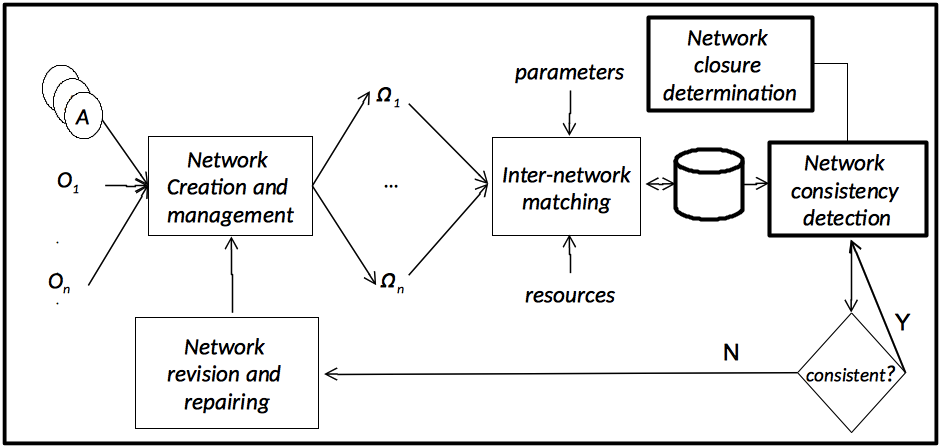
\includegraphics[height=2.2in,width=5in,angle=0]{desafios2c1.png}  
\caption{\small \sl Proposed Challenges adapted from \cite{santospaving}. \label{fig:desafios2a}}  
\end{center}  
\end{figure}

The research addressed initially the investigation conducting a systematic mapping study and comparing with the challenges proposed by Shvaiko and Euzenat \cite{shvaiko2013ontology}. The partial result was a poster at OM2017 \cite{santospaving}. Following an experiment was set to study all the challenges. The first challenge to be investigated is the inter-networking matching (Fig \ref{fig:desafios2a}).

However, when we went deeper investigating these challenges, we realized the need for network closures in order to obtain a response to consistency check or to be able to reason over the structure. Moreover, the determination of closures inside and among networks, by itself, is a challenge that can be explored.  So we modified the figure presented in \cite{santospaving} and include the closure determination as a challenge. (Fig \ref{fig:desafios2a}). 
\end{comment}

\section{Problem Definition} \label{subsec:motivationRelevance}
\begin{comment}
This Section presents the required definitions to formalize and compare the approaches for the inter-network matching problem, which has been recently recognized as a challenge to be explored \cite{santospaving}. 
\end{comment}

A network of ontologies is formally defined as $\Gamma = < \Omega, \Lambda >$, where $\Omega$ is a finite set of ontologies and $\Lambda(O, O')$ is a set of alignments between pairs of ontologies belonging to $\Omega$ \cite{euzenat2015a}. Given a set of two or more networks of ontologies $\Psi$ = \{$\Gamma_1, \Gamma_2,..., \Gamma_n$\}, the internetwork matching problem searches for a final network of ontologies $\Gamma_f$ resulting from the alignments of the networks in $\Psi$. For instance, Figure \ref{fig:interNoN} depicts two networks of ontologies, each one with 3 ontologies, describing two Systems-of-Systems. The goal is to match these two networks, finding  a unique network of ontologies.

\begin{comment}
There are two approaches able to address the inter-network matching problem.  The first one, henceforth called \emph{inter-network pairwise matching}, tries to match each ontology from each network using a basic pairwise approach, which in the end prone duplicate alignments. The second one, henceforth called \emph{inter-network holistic matching}, uses the same strategy described in \cite{megdiche2016extensible} but now applied to networks and searches for the final network considering all the networks at once.
\end{comment}
One of the approaches for matching networks of ontologies is pairwise. Given a set of networks of ontologies, the pairwise internetwork matching sequentially computes the alignment of each pair of ontologies from each pair of networks from this set. For example, given two networks of ontologies $\Gamma = < \Omega, \Lambda >$ and $\Gamma' = < \Omega', \Lambda' >$, in which $\Omega = \{O_1, O_2\}$ and $\Omega' = \{O_3\}$\todo{of Figure \ref{}}, the pairwise internetwork matching is obtained by computing $(((O_{1} \times O_{2}) \cup (O_{1} \times O_{3})) \cup (O_{2} \times O_{3}))$. That is, the pairwise internetwork matching approach computes all matchings between all pairs of ontologies inside each network that is being aligned.  

\begin{comment}
\begin{definition} [pairwise inter-network matching]
\label{def:pairwiseInterNetwork}
Given a set of two or more networks of ontologies $\Psi$ = \{$\Gamma_1, \Gamma_2,..., \Gamma_n$\}, %where $\Gamma$ is a network with $|\Omega| \geq 2$, 
a pairwise inter-network matching obtains %$\Phi$ by checking, 
$\Gamma_f$ by successively aligning every possible pair of ontologies $O_m$, $O_n$, where $O_m \in \Omega_i$ and $O_n \in \Omega_j$ (\{$((\Omega_{1}$ X $\Omega_{2})$ X $\Omega_{3})$ X … X $\Omega_{n}\}$ where $\Omega_i \in \Gamma_i$).


\todo[inline]{essa definicao parece incompleta. FM - Mexi.}
\end{definition}


\begin{figure}[H]
\begin{center}  
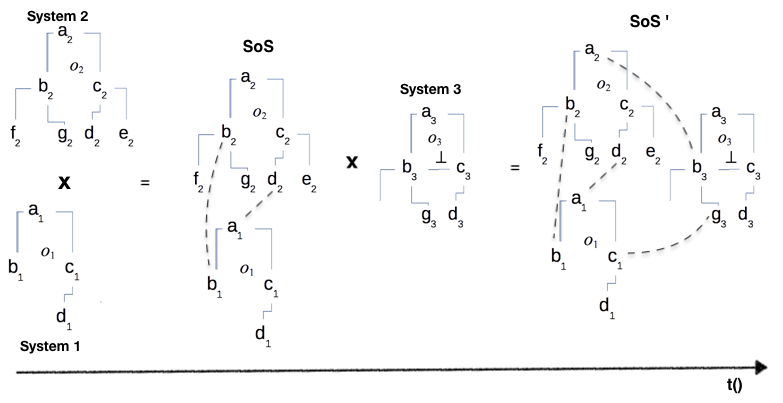
\includegraphics[height=2.6in,width=5in,angle=0]{NoNPair2b.png}  
\caption{\small \sl pairwise inter-network ontology matching  \label{fig:NoNPair}}  
\end{center}  
\end{figure} 
\end{comment}
%FB: retirei este paragrafo
%Since may have equal ontologies composing $\Omega_{1} , \Omega_{2} , ..., \Omega_{n}$, it is possible to find same alignments in some steps. Hence after a merge we need an algorithm that computes if $S \cap (\Lambda 1 \cap \Lambda 2 \cap ...\cap \Lambda n) \not= \{\varnothing\}$. If so then remove the intersection. Consequently  we will compute S = $\{((\Omega 1 X \Omega 2) X \Omega 3) X … X \Omega n - (\Lambda 1 \cap \Lambda 2 \cap ...\cap \Lambda n) \}$


%\subsection{Pairwise weakness } \label{subsec:weakness}

Networks frequently have isomorphisms and trivial alignments that may cause the pairwise approach to find the same alignments more than once, thus requiring an additional step to merge the resulting matches at the end. In the case of isomorphisms, identical correspondences between same entities may be generated (for instance, in Figure \ref{fig:interNoN} a matcher tool may find  $A_{1,1'} = \{<O_1.a_{1}, O_1'.a^{'}_{1}, = >, <O_1.b_{1}, O_1'.b^{'}_{1}, = >\}$). The case of a trivial alignment occurs when a group of entities, that was previously aligned in a network, appears in another network. For instance, a pairwise matcher that receives the networks $\Gamma$ and $\Gamma'$ \todo{(fig \ref{fig:interNoN)}} and has previously computed the intra-network alignments $A_{1,2} = <O_1.b_{1}, O_2.d_{2}, \sqsubseteq>$ and $A_{1',2'} = <O_1'.b^{'}_{1}, O_2'.d^{'}_{2}, \sqsubseteq>$ will work unnecessarily to produce $A_{1,2'} = <O_1.b_{1}, O_2'.d^{'}_{2}, \sqsubseteq>$ and $A_{1',2} = <O_1'.b^{'}_{1}, O_2.d_{2}, \sqsubseteq>$, which are trivial alignments.

The main weakness of pairwise approach is the number of comparisons needed to compute all alignments and the lack of ability to handle isomorphisms and intra-network alignments. 

\begin{figure}  
\begin{center}  
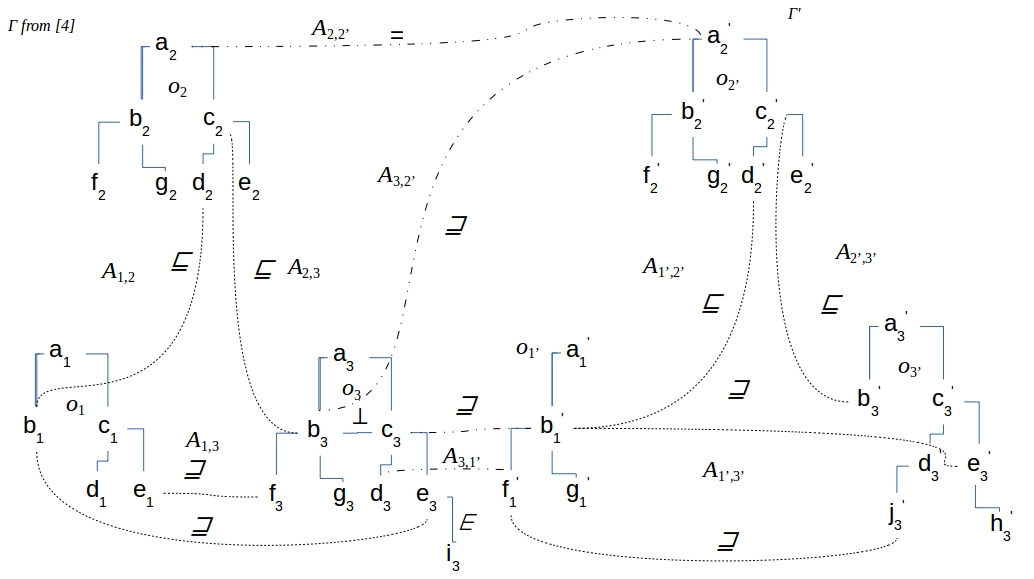
\includegraphics[height=2in,width=4in,angle=0]{NoNExample4.png}  
\caption{\small \sl Internetwork matching of networks $\Gamma$ and $\Gamma'$.\label{fig:interNoN}}  
\end{center}  
\end{figure}

\begin{comment}
\begin{table}[h!]
  \begin{center}
    \caption{Weakness - Pairwise.}
    \label{tab:week}
    \begin{tabular}{l|c|c} 
      \textbf{factor} & \textbf{pairwise} \\
      \hline
      Number of comparison & $\Omega$ X $\Omega'$ \\
      Merge the results  & No  \\
      Deal with intra-network alignments  & No \\
     	Deal with isomorphism  & No \\
    \end{tabular}
  \end{center}
\end{table}
\end{comment}

\begin{comment}
Pairwise approach has to check for each existing entity and need to merge the result at the end of the process. It will match again the intra-networks alignments (the alignments between a pair of ontologies in the same network) and isomorphisms. 
\end{comment}
\todo{Fabio, é nessa seção que você precisa explicar em detalhes as duas abordagens e ilustar com as figuras. Movi elas para cá, mas você tem que incluir o texto explicativo.}
\todo{FB: fabio, eu ja havia apontado isso em outra revisao... tente evitar o estilo de "contagem de historia"no texto, seja mais direto (Algo como "This Section presents the required definitions to formalize and compare the approaches for internetwork matching")}
 
%In order to clarify and go deeper in challenges proposed in \cite{santospaving}, we started to write a formal definition about the matching between two networks of ontologies called inter-network matching. So we first looked out to a start point to anchor our fundamentals. The choose the work of Euzenat \cite{euzenat2015a} as a base of a reliable knowledge. There he defines deeply the concepts of those networks and defines a set of belief revision operators. 


%\subsection{Inter-network alignments} \label{subsec:inter-network}
%\todo[inline]{Esse paragrafo esta muito confuso. Não entendi e assim nõa consegui alterar. Qual? o de cima ou esse de baixo. O de cima estou querendo dizer que estou continuando as challenges e usando a notação do euzenat. O de baixo estou dizendo que cada lainhamento cria uma constraint. Podem sair os 2 e começar as definições direto?}
%Alignments express relations between entities through a finite set $\Theta$ of relations which are independent of ontology relations \cite{euzenat2015a}. The alignment semantic may be constrained when included in a network. In fact when submitted to a set of ontologies,  and a set of alignments, an alignment A must respect all the rich semantic made available by the structure of face consistency problems. To reach this point we need some definitions.

\section{Proposed Approach}
\label{subsec:proposed}

Given the limitations discussed in Section \ref{subsec:motivationRelevance}, we propose SubInterNM, a new subsumed approach for the Internetwork matching problem. SubInterNM avoids unnecessary computation by identifying and reusing trivial and subsumed alignments already computed in the networks of ontologies that are being aligned. In such cases, as the intersection among the networks becomes larger, the set of evaluated correspondences during the alignment process tends to get smaller. %This is possible to occur in some scenarios we discussed in section \ref{sec:introduction}. 

For instance, consider the example depicted in Figure \ref{fig:interNoN}. The networks $\Gamma$ and $\Gamma'$ were aligned using an internetwork matcher. Since $O_{2}$ and $O'_{2}$ are identical, they do not need to be exhaustively compared. Also, both pairs of ontologies $O_{1}$ and $O'_{1}$ and $O_{3}$ and $O'_{3}$ share some subset of entities, thus common parts could be eliminated to compute the final network of ontologies resulted from the internetwork matching problem scenario.

\begin{comment}
Our proposed SubInterNM approach keeps preexisting intra-alignments  intact. Moreover, preexisting inter-network alignments (the alignments between ontologies from distinct   networks) may also be passed as input to our approach so that  only new alignments need to be computed during the inter-network matching process. However, it is possible to do all matches (intra-network and inter-network) again as well. It can be necessary if one has to check for updates on the networks. After subsumed approach eliminates unnecessary pairs, it must use a batch process to align the remaining pairs.
\end{comment}
%\subsection{Implementation} \label{subsec:implementation}
%\todo{referência. O resto é constatação do artigo}


Casanova et al. \cite{casanova2012operations} proposed operations over lightweight ontologies. They define lightweight ontologies as ontologies restricted to DL-Lite core with arbitrary number restrictions. They use a MEG (minimal equivalent graph) approach to create a constraint graph in polynomial time if the graph is acyclic. If the graph is complete, then the problem is NP-Hard. To avoid that, a normalization step is conducted to simplify the graph structure and keep them lightweight. 

Our proposed approach SubInterNM uses a combined set of lightweight operations from \cite{casanova2012operations} to verify the existence of isomorphisms. We extrapolate the original idea to use in networks environments, instead of just single ontologies.

\section{Preliminary Results} \label{sec:results}   

\begin{comment}
We aimed to avoid some unnecessary computation, using the subsumed approach. Hence, we started comparing the pairwise and subsumed approaches. So we measured the number of pair evaluations each approach needed to match the networks. We used some ontologies available inside OAEI initiative dataset in order to help check the results. Therefore we set the experiment to compute the alignments from two networks, we will define, using the following ontologies: cmt, conference, sigkdd, dblp and ekaw.
\end{comment}
Our proposed approach was evaluated in a preliminary experiment using ontologies from the OAEI conference dataset. We experimented 5 distinct scenarios, and in each of them we specified two networks of ontologies to be aligned. The experiments were defined by increasing  the number of ontologies in the network, as well as varying the ontologies and the number of common ontologies between the networks, in order to assess how well our approach would handle the existence of trivial and subsumed alignments:
\begin{itemize}
  \item 2x2: $\Omega$ = \{conference, cmt\} and $\Omega'$ = \{cmt, sigkdd\};
\item 3x2: $\Omega$ = \{conference, cmt, ekaw\} and $\Omega'$ = \{cmt, sigkdd\};
\item 3x3: $\Omega$ = \{conference, cmt, ekaw\} and $\Omega'$ = \{cmt, sigkdd, conference\};
\item 4x3: $\Omega$ = \{conference, cmt, dblp, ekaw\} and $\Omega'$ = \{cmt, sigkdd, conference\}; 
\item 4'x3: $\Omega$ = \{conference, cmt, edas, ekaw\} and $\Omega'$ = \{cmt, sigkdd, conference\}. 
\end{itemize}
 
In order to compare our proposed SubInterNM approach against the pairwise internetwork matching approach, we implemented the pairwise approach using the existing matching system ALIN \cite{da2017semantic} in all experiments. ALIN was selected due to the good results achieved on OEAI 2017, and due to our access to the code \cite{da2017alin}. To use ALIN as a \emph{blackbox} (i.e., without having to change its code), for each internetwork matching experiment, we built all the pairs of ontologies to be aligned and interactively invoked ALIN. 
\begin{table}[h!]
  \begin{center}
    \caption{Total number of comparisons computed by each approach}
    
    \label{tab:results}
    \begin{tabular}{c|c|c|c} 
      \textbf{Experiment} & \textbf{Pairwise} & \textbf{SubInterNM} & \textbf{\% of reduction} \\
      \hline
      2x2 & 14,138 & 5,608 & 60.3\\
      3x2 & 22,236 & 10,027 & 54.9\\
      3x3 & 38,893 & 27,039 & 30.4\\
      4x3 & 42,319 & 27,039 & 36.1\\
      4'x3 & 57,497 & 43,420 & 24.4
    \end{tabular}
  \end{center}
\end{table}
SubInterNM was implemented using operations defined by Casanova et al. \cite{casanova2012operations}, initially considering only the isomorphisms. After, the ALIN matching system\cite{da2017semantic} was also invoked to compute the alignments between the results from $\Omega$ and $\Omega^{'}$. So we computed: 

$\Omega $ as $ O_{1} \cup O_{2} ... \cup O_{n} - O_{1} \cap O^{'}_{1} - O_{1} \cap O^{'}_{2} - ... - O_{n} \cap O^{'}_{n}$  

$\Omega^{'} $ as $ O^{'}_{1} \cup O^{'}_{2} ... \cup O^{'}_{n} - O^{'}_{1} \cap O_{1} - O^{'}_{1} \cap O_{2} - ... - O^{'}_{n} \cap O_{n}$  

Table \ref{tab:results} shows the number of pairs analyzed (i.e., comparisons) by pairwise and subsumed approach to compute alignments in each experiment.
It is possible to verify that SubInterNM reduces the number of comparisons needed to the matching process by at least 24\%, therefore representing a successful way to deal with large networks in the internetwork matching problem. 

Future work will try to reduce even more the number of comparisons with the detection of intra-network alignments. All the data gathered in the experiment is available at (https://bit.ly/2M3jIYS).

%In opposition with alin, used to do the pairwise matching, that is a mature tool and optimized with multi-thread programming, our very first implementation run everything in line. Hence we can optimize, running some code in parallel, using threads or cloud computing. For instance, the union step for each network can run in parallel, all the intersection step can run in parallel and the difference step can also run in parallel for each network, as well. So probably if you increase the number of networks, you will increase the chance of having more subsumed networks and consequently reduce the processing. Although intersections may grow substantially, they not seen to be a problem as they can be all parallelized.

%The load and union phase is the bottleneck. During the load the tool have to construct the graph for the entire structure, the constraint graph and normalize everything to create the lightweight representation. We are doing loads and unions together and usually this phase could be done before the need of alignments. Even if you have only the structures created the result could be better. We measured the loading phase of each ontology and cmt, for instance, was loaded up to 55s 384ms, showing the union is not the villain of the process. Indeed it reveals if our ontologies graphs were ready in our tool we could run union only when the align process begins. This avoids running union at each update on the structures. We must separate load from the union.

\begin{comment}
We also have to mention that after the matching process using the pairwise way, we need to eliminate duplicate alignments. Hence, the pairwise approach has more work to do after finish the match phase. 
The comparison between our subsumed approach and the holistic inter-network matching is also planned. 
\end{comment}
%We are finishing our merge tool and we could not compute this time in this experiment. We expect to do it soon as future work. Finally, our approach runs a minimize function that clear duplications at each step. We can move it only to the end of the process or simply run the merger tool we are developing.    

\begin{comment}

\end{}
\section{Related Work} \label{sec:related}
\todo[inline]{FM - não mexi aqui, pois não sei o que fazer! Falar de novo de pairwise e holistic aqui me parece repeteco. Só se eu pegar a parte de implementação e jogar aqui. O que acham?}
\todo[inline]{FB: eu acho que pode sair}
There is not so much in this research area to compare. So we went a lit bit more in abstraction to check some interesting ideas to use in future.  
The work of \cite{kermarrec2007gossiping} uses a gossiping algorithm that regularly each peer picks up some other peer for a two-way information exchange. Each peer selects some correspondences to send to another peer. This process broadcast increasing the knowledge around the network without the need of translate queries at each peer. Despite they have to walk through all structure gathering information, the alignments between networks may be constructed same way step a step, according to the progress of the two-way exchange. The main difference is: they avoid a huge processing step of matching several ontologies and networks at once. 

In \cite{euzenat2014c} Euzenat created a game and use agents to repair alignments over a network. The algorithm repair using one of three modalities: delete, add or replace. So the hypothesis of an agent acting locally and without a global knowledge can repair alignments is confirmed, but this does not replace the need for repair techniques. Although our approach does not embrace the repair of alignments, the way the agents communicate each other and determine the repair actions may be used to create a background knowledge and avoid some alignments do be processed later by a matcher. 

\end{comment}
\section{Conclusion} \label{sec:future}

This work addressed the problem of internetwork ontology matching, a natural evolution of the classical ontology matching problem for highly interconnected scenarios of Systems of Systems, which are of increasing popularity and relevance. 
We proposed SubInterNM, an approach for internetwork ontology matching that optimizes the required computation of correspondences by identifying and reusing trivial and subsumed alignments. Preliminary evaluation results showed the potential of the approach and opportunities for improvement, in scenarios using lightweight ontologies. The computation of subsumed networks posed an overhead computation since it is a well-known NP-Hard problem \cite{hsu1975algorithm}. Therefore, further implementations may compute trivial alignments, using it as background knowledge for the matching process \cite{shvaiko2013ontology}. 

In future work, we expect to improve our implementation, including parallel programming and infrastructure. We also plan to move forward exploring trivial alignments in newer versions of the tool. 

%The alignment API \cite{david2011alignment} have some operations over networks, including matching, invert, trim, normalize and close. The API is very well implemented and have some documentation to help users use and install. However, developers need a lit bit more documents to understand and use without reading every command in available code. The management infrastructure, on the other hand, may be used to our explore our challenges without so much effort. We are planning to check if the tool is easy to extend to be used as a background server to our challenges.     

\bibliography{bibliography}

\end{document}
